In this section, we present our measurement methodology along with the
metrics  considered  and  discuss about  the  performance-power-energy
trade-off of the model system on the different platforms stated.

\subsection{Measurement methodology}
\label{subsec:4.1}

We  approach  the  assessment  of  the energy  footprint  and  overall
performance    of    \cosmoart    with    two    important    metrics:
\textit{time-to-solution} (TTS) and \textit{energy-to-solution} (ETS).
TTS refers to  the total wall clock time  of the application execution
time. ETS  is the amount of  energy spent to  achieve results.  Energy
consumption is  assessed by sampling the power  during execution which
is then averaged and multiplied  by the TTS to determine ETS. Whenever
possible, multiple  production runs  were performed to  illustrate the
reproducibility  of   the  baseline,  and   quantify  the  significant
uncertainties in  the power measurement, as dictated  by the available
technology.

For  the   experiments  on  \tinto  platform,  we   also  analyze  the
contribution of the MPI library  to the energy consumption and how the
use  of  the aggressive and degraded message-passing progression engine 
policies can potentially  render energy  savings.

Specifically,   the  OpenMPI 1.6.5  library,  features  two  operation 
policies, \emph{aggressive} and \emph{degraded}, which can be  selected 
before \cosmoart is launched. In the \emph{aggressive} (default) policy,  
normally used in exactly- or under-subscribed mode  (i.e., the  number 
of running processes is equal to or less than the number of  available 
cores), MPI processes will never voluntarily give up the processor  to 
other processes. With some network transports, OpenMPI processes  will 
spin  in  tight  loops  attempting  to  make message passing progress, 
effectively causing other processes to not get  any  CPU  cycles  (and  
therefore never make any  progress).  This  usually  yields  the  best 
performance but high CPU utilization, possibly at the cost of a higher 
energy usage.  On the other hand, the \emph{degraded} policy, suitable 
for the oversubscribed mode (i.e., more  processes  are  running  than 
total cores  available),  MPI  processes  will  frequently  yield  the 
processor to its peers, thereby allowing all processes to make progress. 

In our experiments with \cosmoart only the exactly-subscribed mode  is
used. Therefore, \cosmoart processes running  in  the  \emph{degraded} 
policy are constantly checking for the completion  of  an  event (e.g. 
send or receive) and repeatedly calling to  \texttt{sched\_yield()} to 
be picked again by the Linux scheduler. Although one can expect no benefits 
from   using   the  \emph{degraded}   policy   compared   with     the 
\emph{aggressive} one, notable differences can be observed in the CPU utilization. 
In a separated  test  with  the  \emph{aggressive}  policy 
enabled, we noticed that a blocked MPI process waiting for an incoming 
message has CPU utilization of 100\,\%,  however  when  the \emph{degraded} 
mode  is  set,  the  CPU  utilization is only $50\,\%$, approximately. 
Although neither of both policies avoid busy-waiting loops in blocking 
routines, the use of the \emph{degraded} policy is as much as we can 
do in OpenMPI to reduce the CPU utilization, and thus save energy.

% polling configuration
% (the default mode) ``MPI''  continually polls the network interface to
% check for  the completion  of an event  (e.g. send or  receive).  This
% usually yields  low latency  but high CPU  utilization. Thus,  one can
% expect that  this mode attains  the best performance, possibly  at the
% cost a higher energy usage. In  the blocking mode, the CPU is yield to
% other     processes/threads    if     there     are    no     incoming
% messages~\cite{Castillo-2012}.

\subsection{Time-power-energy analysis}
\label{subsec:4.2}

Figures~\ref{fig:1} and \ref{fig:2}  account respectively for \monch's
Isola  E1 Rack 2  and \pilat'  Isola HD  total power  measurements for
1-day or 2-day simulations. On \monch, the 1-day simulation was issued
only twice due  to usage restrictions.  As time  resolution was set to
one  update every  5 minutes  for power  sampling, the  averaged power
consumption was computed by considering  6 values for each single run.
On \pilat, the 1-day simulation was  issued four times and a 2-day run
only once.  Similarly, the  averaged power consumption was computed by
considering 4  values for each single  1-day run and 9  values for the
2-days run. Corresponding results are gathered in Table~\ref{tab:1}.

\begin{figure}[htbf]
  \centering
  \includegraphics[width=0.48\textwidth]{Figs/NRJ_benchmark_Monch.eps}
  \caption{Isola E1 Rack 2 total power of \monch.}
  \label{fig:1}
\end{figure}

\begin{figure}[htbf]
  \centering
  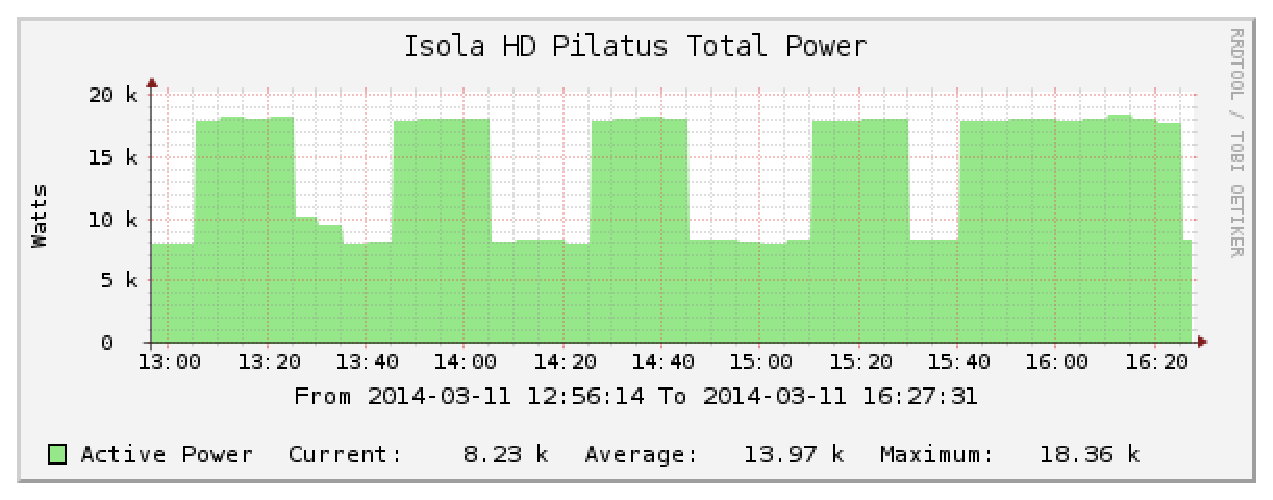
\includegraphics[width=0.48\textwidth]{Figs/NRJ_benchmark_Pilatus.eps}
  \caption{Isola HD total power consumption of \pilat.}
  \label{fig:2}
\end{figure}

\begin{table}[htbf]
  \centering
  \caption{Averaged power consumption (W) of the platforms.}
  \label{tab:1}
  \begin{tabular}{cccc}
    \hline\noalign{\smallskip}     \textbf{\scriptsize{PILATUS}}     &
    \textbf{\scriptsize{MONCH}}  &  \textbf{\scriptsize{TINTORRUM}}  &
    \textbf{\scriptsize{TINTORRUM}}           \\          &          &
    \textbf{\scriptsize{(\emph{Aggressive})}} & \textbf{\scriptsize{(\emph{Degraded})}}
    \\    \noalign{\smallskip}\hline\noalign{\smallskip}   18035.0   &
    12622.5 & 3713.6 & 3651.8 \\ \noalign{\smallskip}\hline
  \end{tabular}
\end{table}

In  Figure~\ref{fig:3}, we  compare both  TTS (right  Y-axis)  and ETS
(left  Y-axis)  metrics  on  both  platforms.  As  expected, Intel Sandy Bridge EP processors of \pilat
outperform the Intel Ivy  Bridge EP processors of \monch, being roughly 130\,\%  faster.  The reason
for that is two-fold: \emph{i}) they have higher clock frequency than Ivy
Bridge  (2.6\,GHz  against  2.2\,GHz),   and  \emph{ii})  they  aim  at
computing   speed  regardless   to  be   energy  efficient.    In  our
experiments,  \monch  showed  the  best  energy-to-solution,
reducing the energy consumption of \pilat by approximately 7\,\%.

Averaged TTS and ETS results  over 10 repetitions of 24h simulation on
\tinto are shown in  Figure~\ref{fig:4}. The corresponding results for
the  averaged total  power are  also shown  in  Table~\ref{tab:1}.  As
expected, the average total power consumption by \cosmoart while using
the \emph{degraded} MPI policy is about  2\,\% less than that consumed by the
\emph{aggressive} one. This is  due to  the reduction of CPU usage (of about 50\,\%) while using  the \emph{degraded} MPI policy, in
contrast with the \emph{aggressive} policy that always yields to 100\,\% of CPU utilization while waiting for an incoming message. From the point of  view of the execution time, there is a
slight reduction  for the \emph{degraded} MPI  policy. One can  expect that the
costs of the context switches produced in the \emph{degraded} MPI policy can lead to
an  increase  of  the   execution  time,  however,  applications  with
extensive computing,  as e.g.  \cosmoart, may show  better performance
with the \emph{degraded} policy. This effect works in  favor with our results
since the energy consumed is also reduced (2\,\%) just by changing the
behavior of the OpenMPI library  to the \emph{degraded} policy, i.e, with the
\texttt{--mca    mpi\_yield\_when\_idle 1}   parameter   set    in   the
\texttt{mpirun} command.

\begin{figure}[htbf]
  \centering
  \includegraphics[width=0.5\textwidth]{Figs/Time_E2S_COSMO-ART-0.eps}
  \caption{Time-to-solution and  energy-to-solution comparison between
    \pilat and \monch for a 24h simulation.}
  \label{fig:3}
\end{figure}

\begin{figure}[htbf]
  \centering
  \includegraphics[width=0.5\textwidth]{Figs/Time_E2S_COSMO-ART-1.eps}
  \vspace{-1cm}
  \caption{Mean time-to-solution and  energy-to-solution on \tinto for
    a 24h simulation using the  \emph{aggressive} and \emph{degraded} MPI policies. The
    95\,\%  confidence  intervals of  Student's  $t$ distribution  (10
    samples) clearly  indicates an improvement for the \emph{degraded} policy in
    both TTS and ETS.}
  \label{fig:4}
\end{figure}

\begin{figure*}[ht]
  \centering
  \hspace{0.8cm} \scalebox{0.62}{\input{Figs/24hour.pstex_t}}
  \caption{24  hours  simulation power  trace  using  the \emph{aggressive}  and
    \emph{degraded} MPI policies on \tinto.}
  \label{fig:5}
\end{figure*}

\begin{figure*}[ht]
  \centering
  \scriptsize
  Simulation of 1 hour during midday (11h--12h) using the \emph{aggressive} MPI policy \\
  \scalebox{0.5}{\input{Figs/11_12_blq0_figure.pstex_t}} \\
  Simulation of 1 hour during midday (11h--12h) using the \emph{degraded} MPI policy \\
  \scalebox{0.5}{\input{Figs/11_12_blq1_figure.pstex_t}} \\
  1 hour simulation during midnight (23h--24h) using the \emph{aggressive} MPI policy \\
  \scalebox{0.5}{\input{Figs/23_24_blq0_figure.pstex_t}} \\
  1 hour simulation during midnight (23h--24h) using the \emph{degraded} MPI policy \\
  \scalebox{0.5}{\input{Figs/23_24_blq1_figure.pstex_t}} \\
  \begin{tabular}{rlp{-0.2cm}rlp{-0.2cm}rlp{-0.2cm}rlp{-0.2cm}rl}
    & &  & &  & &  \\[-0.15cm]
    Computation     & \multicolumn{1}{>{\columncolor[RGB]{  0,  , 255}}p{0.4cm}}{} & & 
    Block. send     & \multicolumn{1}{>{\columncolor[RGB]{255,  0,174}}p{0.4cm}}{} & & 
    Synchronization & \multicolumn{1}{>{\columncolor[RGB]{179,  0,  0}}p{0.4cm}}{} & & 
    Wait/Wait all   & \multicolumn{1}{>{\columncolor[RGB]{235,255,  0}}p{0.4cm}}{} \\
    & &  & &  & &  \\[-0.15cm]
    Immediate recv. & \multicolumn{1}{>{\columncolor[RGB]{100,100,177}}p{0.4cm}}{} & &
    Waiting a msg.  & \multicolumn{1}{>{\columncolor[RGB]{255,  0  ,0}}p{0.4cm}}{} & & 
    Group comm.     & \multicolumn{1}{>{\columncolor[RGB]{255,144, 26}}p{0.4cm}}{} & &
    Others          & \multicolumn{1}{>{\columncolor[RGB]{192,224,  0}}p{0.4cm}}{} \\
    %I/O             & \multicolumn{1}{>{\columncolor[RGB]{172,174, 41}}p{0.4cm}}{} & &
    %
    %Idle            & \multicolumn{1}{>{\columncolor[RGB]{117,195,255}}p{0.4cm}}{} \\
  \end{tabular}
  \caption{Power-performance   traces  during   midday   and  midnight
    leveraging the \emph{aggressive} and \emph{degraded} MPI policies on \tinto.}
  \label{fig:6}
\end{figure*}

\subsection{Power-performance profiling and tracing}
\label{subsec:4.3}

A full tracing  experiment is conducted on \tinto  in order to capture
an overall power profile at a much finer resolution using the attached
PDUs in each  node. First we run \cosmoart for  a 1-day simulation and
analyze the  power consumption.  Second we  correlate performance with
power  traces  of  two  1-hour  time frames  during  the  day:  midday
(11h--12h) and midnight (23h--24h). All the experiments on \tinto were performed
using 192 cores with 12 MPI processes per node, i.e., using an exactly-subscribed MPI mode.

In order to obtain an initial overview of the power consumption of the
system  model,  we  obtained  power  profiles  leveraging  our  \pmlib
power-measurement    framework   over    a    1-day   simulation    of
\cosmoart. These profiles, produced with both \emph{aggressive} and \emph{degraded} MPI
policies,  are depicted in  Figure~\ref{fig:5}. The  first observation
for the \emph{aggressive} MPI policy is that the first and last hours of the day
consume slightly less  power than the midday hours.  We relate these
variations  due   to  the  different   chemical  reactions,  aerosols,
radiations  and clouds  formation processes,  computed by  ART, taking
place during  daylight hours  but not during  night. In this  case the
peak power consumption is about  3821\,W. Looking at the power profile
using the \emph{degraded}  MPI policy, we observe that  the 1-hour pattern is
repeated along  the 24-hours, favoring  the reduction of  power during
night  hours in  a  more noticeable  way  than that  with the   \emph{aggressive}
policy.   The peak  power consumption  during day  hours  while the
 \emph{degraded}  MPI policy  is leveraged  is  about 3768\,W,  which means  a
reduction of around  50\,W with respect to the  \emph{aggressive} mode. Also, we
notice systematic  power drops for each simulated  hour.  We associate
them  to periods  in  which  the processes  were waiting  for
incoming messages  or synchronizations, thus  yielding the CPU  to a lower
usage. Our final observation is the reduction of the TTS by 2\,\% with
respect to the  \emph{degraded} MPI policy.

To  gain  more  insights   about  the  power-performance  behavior  of
\cosmoart,  we  obtained power-per\-for\-man\-ce  traces  to allow  us
correlate  the type  of  tasks  being executed  with  the total  power
consumption  along  the   time  (see  Figure~\ref{fig:6}).   For  this
experiment we  limit the simulation  time to 1 hour  because: \emph{i})
the  pattern of  the computation  performed by  \cosmoart  is repeated
hourly and, \emph{ii}) the weight  of a 1-day simulation trace can not
be easily handled using our  machines and memory available (each trace
file was about 45\,GB). Thus, we shrink the simulations
to 1 hour during midday (from 11h  to 12h) and during
midnight  (from 23h  to  24h), in  which  \cosmoart perform  different
internal computations.  At  the same time we leverage  the two already
stated MPI policies: \emph{aggressive} and \emph{degraded}.

All  the  traces  in   Figure~\ref{fig:6}  are  divided  in  different
computation  phases. In first  phase all  the processes  perform group
communications      and       execute      MPI-receive      primitives
(e.g. \texttt{MPI\_Recv}). The second one performs computation bursts,
combined  in  between   with  group  communications,  blocking  sends,
immediate  receives and  MPI-wait primitives.  Finally,
group  communications interlaced  with computation  and  a significant
synchronization  phase are  performed. From  the performance  point of
view, one can notice a reduction of 2\,\% in the TTS that \emph{degraded}  MPI
mode leads over the \emph{aggressive} MPI  policy. On the other hand an averaged
reduction of power consumption of  2\,\% is attained with the \emph{degraded} 
MPI policy  only in  routines that actually  perform synchronizations,
group  communications  and  MPI-receive/-wait primitives.   Thus,  the
reduction of the power-energy  pair directly depends on the percentage
of time in which blocking MPI  operations are executed. For the 1 hour
simulation traces, an average of 50\,\% of the time the processes were
waiting for incoming messages.  Taking  into account that  the total power  reduction during
blocking phases  is about 5\,\%,  one can compute an  approximation of
the  power savings,  i.e., $50\,\%  \times  5\,\% =  2.5\%$, which  is
consistent  power  reduction  obtained  for  the  full-day  simulation
(around  2\,\%). However,  we  expect higher  power/energy savings  if
upcoming versions of OpenMPI support full blocking policies as well as if 
future architectures tend proportional computing~\citep{Barroso-2007}.

% \begin{figure*}[htbf]
%   \centering
%   Simulation of 1 hour during midnight (from 23h to 24h) leveraging the polling MPI policy\\
%   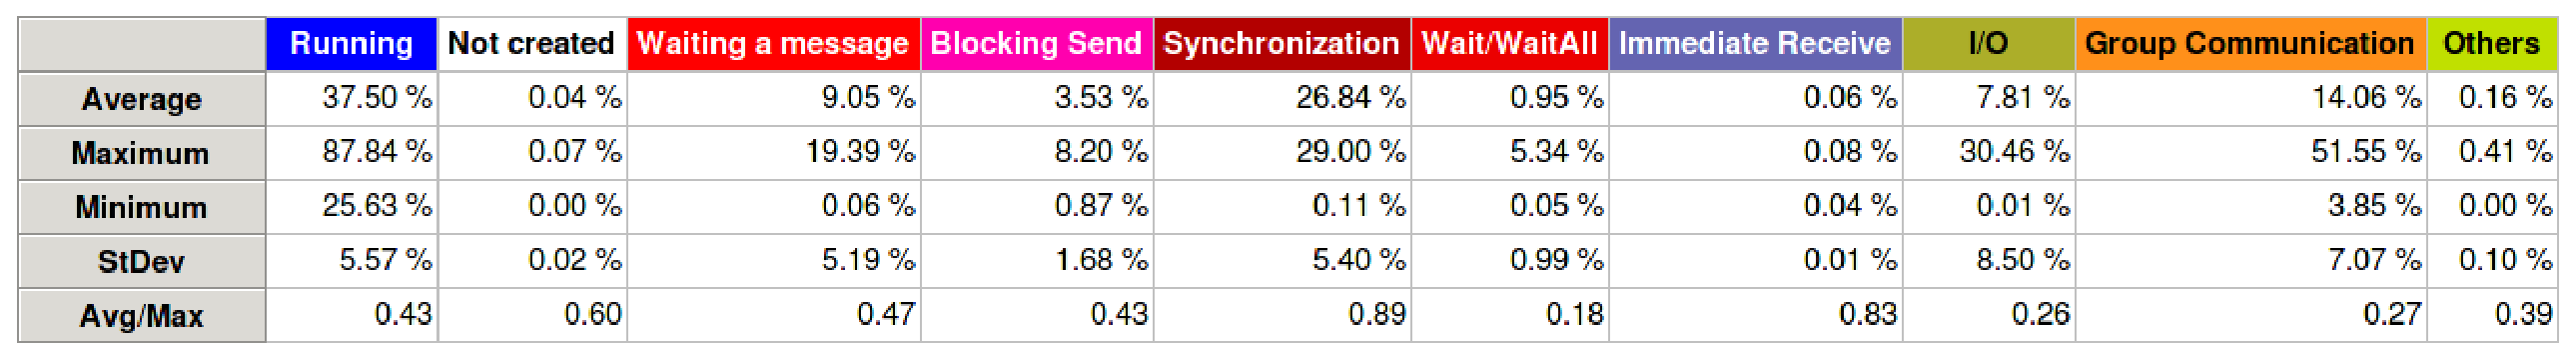
\includegraphics[width=0.78\textwidth]{Figs/23_24_blq0_stat.eps}\\
%   Percentage of time for the 1 hour during midnight (from 23h to 24h) leveraging the polling MPI policy\\
%   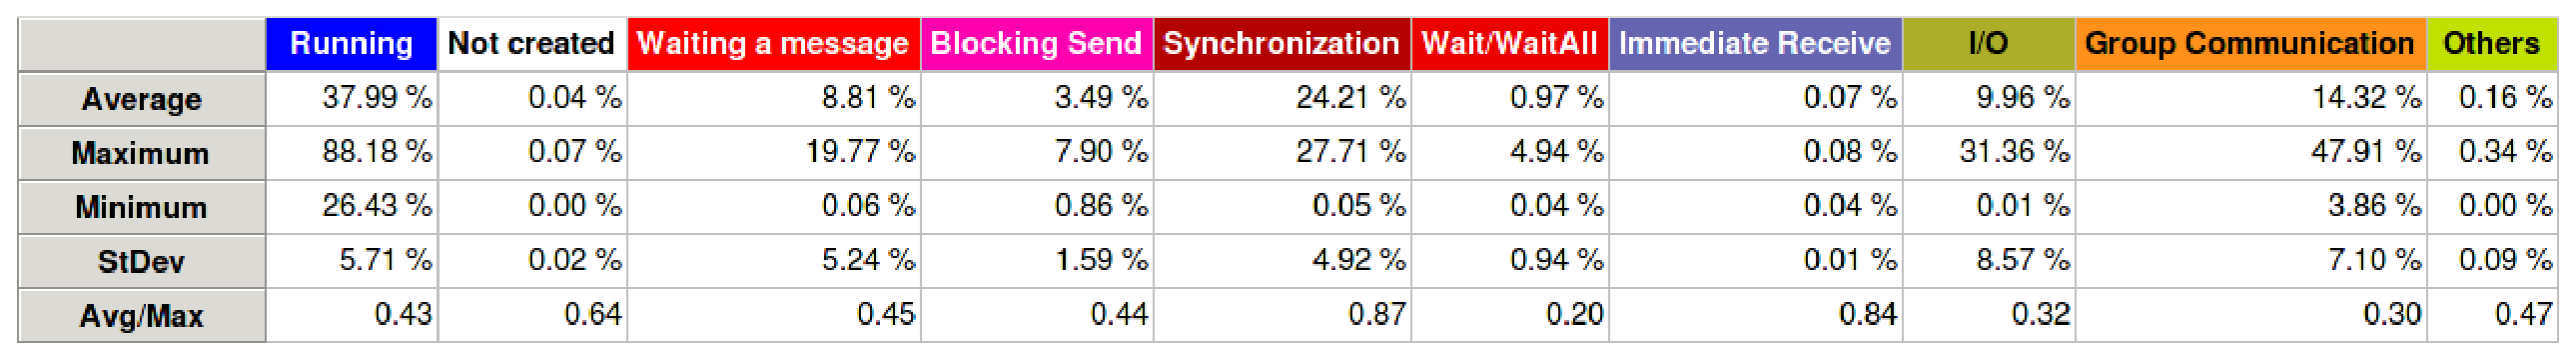
\includegraphics[width=0.78\textwidth]{Figs/23_24_blq1_stat.eps}\\
%   \caption{blabla}
%   \label{fig:7}
% \end{figure*}


